\section{Sensitivity to Error Surface Quality}
In the spirit of the list above provided by \cite{van2007neurofitter}, the next item should be called ``Efficient Convergence", but this efficiency really comes down to the nature of the error surface created by the choice of models, tests, and experimental data.

\subsection{Objective Function Dimensionality vs Model Parameter Dimensionality}
If a given class of models is capable of describing the behavior of a given real neuron, then the number of independent, reliable tests used to generate the objective function can be as large as desired; more tests just provide more information to quickly rule out irrelevant regions of parameter space.
On the other hand if a model class is only capable of describing a fraction of the real neuron's behavior, too many distinct tests will result in an optimization problem that can never be fully satisfied.
Since ``all models are wrong, but some are useful" (Box, 1976), let us imagine that we usually in the latter case.

\subsection{When Does Genetic Optimization Get Stuck?}
Genetic algorithms are known as derivative-free optimizers, since they do not follow any gradient down the error surface, or even know of the existence of such a gradient.
Chromosomes only survive and reproduce differentially according to their location on the error surface.
Thus, genetic optimization is never truly "stuck" inside a local minima on the error surface, as mutation or crossover can always produce new chromosomes outside the basin of attraction.
Despite this robustness, just like in gradient descent, genetic algorithms can only be guided by information in the error surface.
When the objective function has a low-dimensionality, for example when it is based upon tests that mostly compute small variations on the same small number of features of the simulation output, it may not provide enough information to distinguish one location in parameter space from another one close by, even though the first may be closer to the optimal solution than the second.
In other words, many regions of parameter space may be locally flat at a mesoscopic scale, and local minima at a microscopic scale may thus be difficult to escape.
No lower error solution may be available within a reasonable distance (in parameter space) from the current one.
A variety of potential error surfaces are presented in Figure \label{fig:test2}.

\begin{figure}
\centering
      \label{fig:test1}
      \centering
      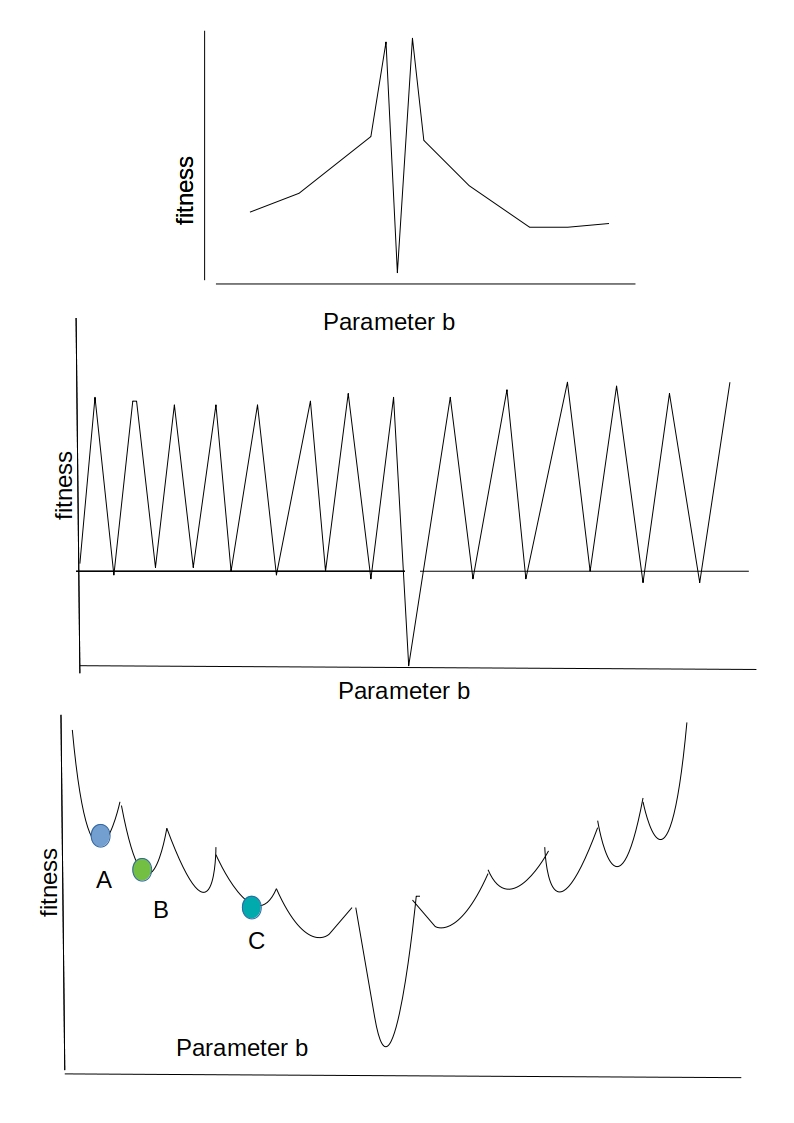
\includegraphics[scale=0.75]{figures/spectrum_worst_error_surfaces2.jpg}
      \caption[Challenging Error Surfaces]{\textbf{Challenging Error Surfaces}. 
      Fitness here should be relabeled "Error".
      The top panel shows an error surface where an optimizer is unlikely to identify the global minimum error.
      Any exploration of the region leading towards that minimum is likely to be abandoned prematurely.
      Only an extremely lucky set of initial chromosomes or a random mutation might result in exploration of the region immediately around the global minimum.
      The middle panel is more hopeful, showing an error surface that does not actively block the global minimum from being explored.
      However, the surface is still mostly uninformative.
      The bottom panel shows a cross-section of Rastrigrin's function (described in the Introduction).
      Despite its hype, this is really the least challenging of the three error surfaces shown here, as there as at least long-range structure to the error surface that a genetic algorithm can exploit.
      }
      \label{fig:test2}
\end{figure} 

\subsection{Defects in the Error Surface}
The real error surfaces that guide optimization here have ``defects", for example discontinuities (due perhaps to bifurcations in the underlying dynamical system, e.g. from spiking to non-spiking) or to deep local minima, that make optimization challenging.
I coined the term ``corrugated" to describe surfaces low amplitude oscillatory disturbances across the error surface.

Some optimization techniques require a perfectly convex error surface to converge.
Genetic algorithms are more tolerant, up to a point, but an extremely high dimensional optimization problem with a large number of optima can still be intractable.
So which error surface defects are truly harmful?
This largely comes down to scale.
The corrugation observed in the error surfaces here was typically on a much smaller scale than the long-range structure that guides optimization.
Consider something analogous to a signal-to-noise ratio (SNR), describing the information that guides optimization vs the wrinkles that impede it.
When SNR is larger, defects are less consequential.
Figure \ref{fig:easy-case} gives an example of an error surface that, while not totally continuous or convex, is nonetheless easily handled by the optimizer.

\begin{figure}      
\centering
      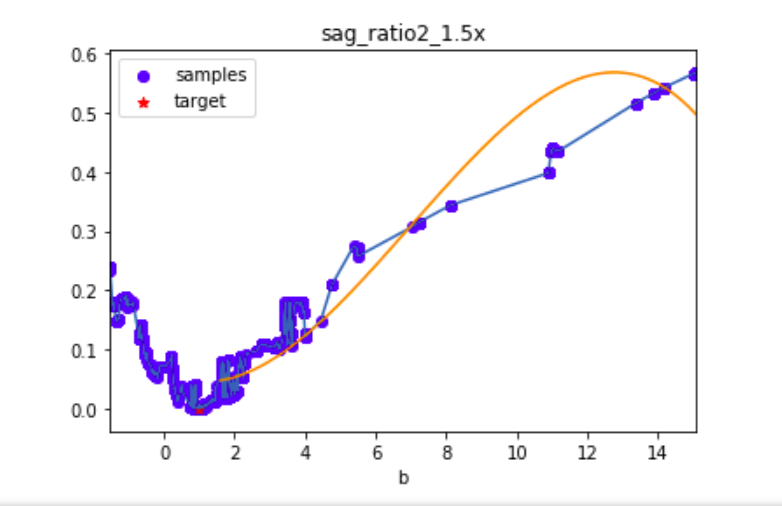
\includegraphics[scale=0.85]{figures/parameter_b_friendly_surface.png}
      \caption[A non-convex but manageable error surface]{\textbf{A non-convex but manageable error surface}.
      The vertical axis shows error (model-data disagreement) for ``sag-ratio" feature computed at 1.5 $\times$ rheobase as the value fo the $b$ parameter in the Izhikevich model is slowly varied.
      The blue dots show the actual error values, and the orange curve shows a low-order polynomoial regression fit.
      While the fit is clearly not perfect, the fact that the error surface can be approximated by a low-order polynomial suggests that it will not be difficult to find the minimum (red dot).}
      \label{fig:easy-case}
\end{figure}

I observed that the NSGA2 selection algorithm was particular vulnerable to defects in the error surface, and required a higher SNR to obtain optimal solutions.
NSGA2 is a fundamentally conservative and short-range approach to evolution, so it may simply lack the drive to escape problematic regions of the error surface.
Unlike NSGA2, IBEA was less sensitive to such defects, and required a lower SNR to converge rapidly. 

However, in any algorithm as the optimum is approached, the rate of mutation must slow down to enable efficient short-range exploitation of the peri-optimum region.
one should not expect to see evidence of efficient-learning. In later stages of This is precisely the phase when the optimizer will be more sensitive to small amplitude corrugations, which become large relative to the small gains to by moving between, say, a parameter set $1\%$ away from the optimum and the optimum itself.

The multiobjective function is derived from the objective functions associated with each feature used in optimization.
As such, the multiobjective function will be more corrugated if more of the component objective functions are corrugated.
Consequently, optimization is more likely to converge if the number of corrguated components is kept to a minimum.
In practice, I observed satisfactory solutions even when only $>\frac{1}{2}$ total number of objectives had no corrugation.
For example, in a four-objective problem, if the $4$th objective is uninformative, but not actively misleading, inclusion of that 4th objective may only slow down the speed of optimizer convergence, but not actually change the final outcome.
By contrast, if that $4th$ objective is actively misleading, the optimizer will likely find a satisfactory (but non-optimal) solution by compromising with the dominant $3$ objective functions.

%\begin{comment}
%\begin{figure}
%\begin{center}
%     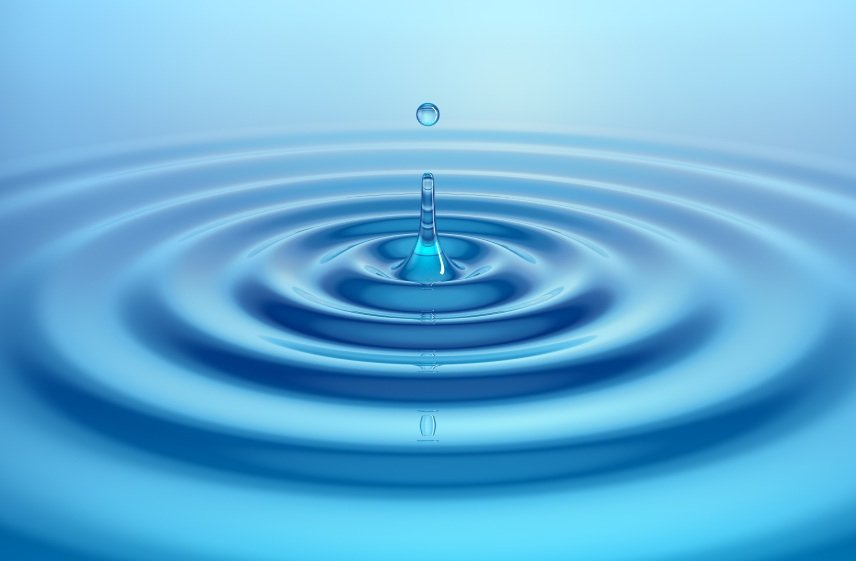
\includegraphics[scale=0.65]{figures/pond_ripple_surface.png}
%     \caption[Conceptualizing moderate to worst case error surfaces]{In the case of pond ripples the cost function is defined so that the maxima is the optimal %location on the surface. Ripples on a body of water are more challenging to optimize, as the water surfaces are approximately flat on the large scale, yet on the small scale maximas will be temporary preoccupy the GAs learning, but outside of those peaks, there is little large scale information to utilize.}
%      
%      \label{fig:test1}
%\end{center}
%
%\end{figure}
%\end{comment}



% Note Help wanted making a professional version, of this known to be unattractive draft/concept figure.
     
      % The second type of error surface actually a 1D (and upside down) cross section of the 2D pond diagram, only actively misleads locally, globally it simply contains no helpful global information. Learning will not be of any assistance in obtaining the optima, but also learning won't be a disadvantage either, the Genetic Algorithm, will simply behave as a random sample testing algorithm, the GA will find the optimum in time, but possibly not as quickly or reliably as exhaustive search would. The second figure is a cross section of the pond ripple argument}







%   When considering 2D relationships between single parameters and single objective functions, ideally each error function might contribute helpful information, which en-masse boosts the total amount of helpful information. For-instance some 2D error mappings, may contain one or more local minima, but in the same region a different error mapping could lack the error well, meaning that at least one out of two error functions contribute incentive to stride across a minima. The mapping that contains wells, might still be useful to guide optimization, as it may also lack minima in regions were the counterpart has them, additionally the alternative mapping may have regions of $~0.0$ gradient where the other mapping contains significant gradient.
   
   % I am not sure if its impossible to make progress.
 %  Through strategy it is possible to optimize satisfactorily without complete prior knowledge of error surfaces, although such a strategy is not recommended. If prior knowledge of an error surface is prohibited, evolutionary algorithms are definitely a more likely to work than gradient descent.
   
   
   % I don't know if this is true:
   % through good luck you could do heaps of optimization, whithout knowing the error surface.
   % It is almost impossible to make progress without some prior knowledge of the error surfaces, as knowledge of the error surface is a prerequisite for constraining optimization. 
   
%   Not all surfaces, provide equally useful information. There are spectrum's of surface quality between convex triangular or parabolic depressions acting as the best solution surfaces, flat functions, and misleading functions. 
   
\subsection{Contingent Discontinuities}
\label{sec:contingent_discontinous}
Some tests used to compute the objective function may depend on the results of other tests.
They may depend on the measured value of one feature, for example, a test of the action potential width at half-height depends on the height measured from threshold which depends on the threshold.
Or they may depend on a stimulus parameter derived from a previous test; for example, computing the first inter-spike interval (ISI) at 1.5x rheobase first requires computing rheobase, and then multiplying the rheobase value by 1.5 to generate the stimulus for the ISI test.
Such an ISI test--and its results--is thus ``contingent" on the results of the rheobase test.
This has confounding implications.
Suppose that as some model parameter $X$ is increased, the cell becomes more excitable.
All things being equal, more excitability would be associated with a lower rheobase, and with a narrower first inter-spike interval at a fixed current.
But because the rheobase determines the value of the actual current injected in the ISI test (i.e. the ISI test is contingent), the ISI could go up or down; it would go down if the direct effect of greater excitability associated with increased $X$ dominates; it would go up if the indirect effect of a smaller current injection dominates.
In fact, it is impossible (or at least impractical) to predict which of these will "win", and the resulting error surface for the ISI test becomes extremely corrugated, as small increments in $X$ cause increases and then decreases in the error of the objective function, with no discernible pattern.

\subsubsection{Examples of Contingent Discontinuities}
Figure \ref{fig:probably_smooth_constraint} provides a concrete example of the discontinuous error surface that results from such contingencies.

\begin{figure}
\centering
      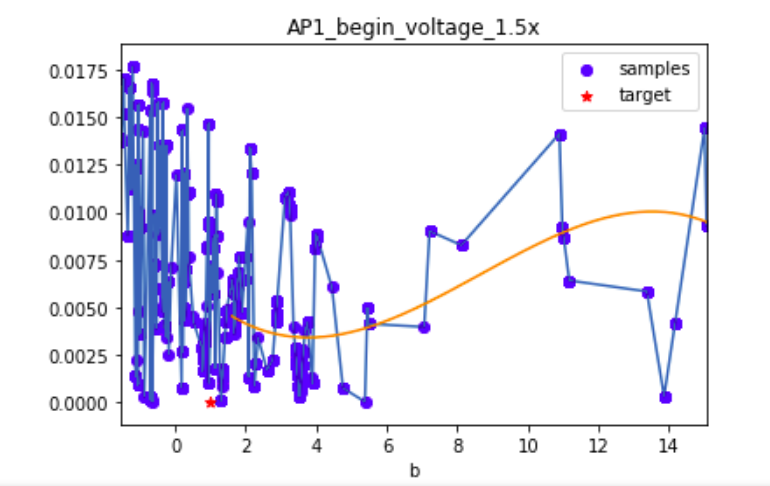
\includegraphics[scale=0.85]{figures/parameter_b_hopeless_surface.png}
      \caption[A non-convex and unmanageable error surface (1)]{\textbf{A non-convex and unmanageable error surface}.
      Similar to Figure \ref{fig:easy-case}, but showing the error in another feature (the membrane potential at the start of the AP waveform) as the same parameter is varied.
      This error surface is extremely corrugated, the polynomial fit has no hope of approximating what is going on for $b<6$, and the optimizer stands little change of finding the global minimum, if such a minimum is even meaningful here.
    }
      \label{fig:probably_smooth_constraint}
\end{figure}

The problem is even more extreme when the contingent test can produce missing values.
For example, an ISI test depends on their being an inter-spike interval to measure, i.e. it requires a second spike to be produced.
If there is no second spike, this test will emit a missing value.
Thus as $X$ is increased, the error surface associated with the ISI test will be pocked with missing values every time the underlying change in excitability is offset too much by the ensuing change in rheobase-derived injected current.
An example of this even more challenging case is given in Figure \ref{fig:discontinuous_constraint}.

\begin{figure}
      \centering
      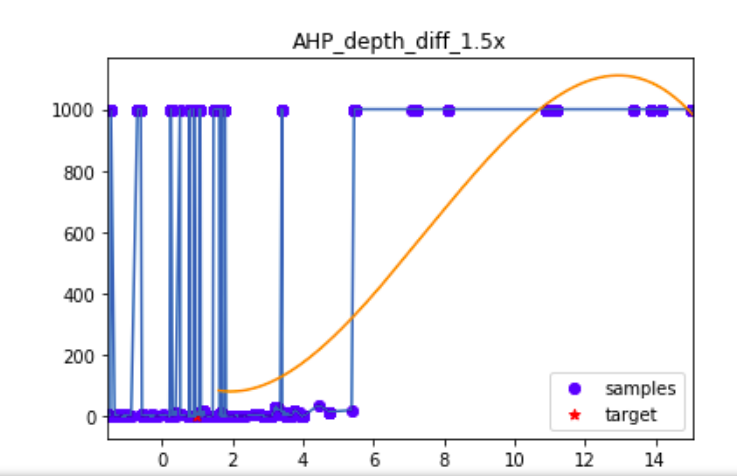
\includegraphics[scale=0.85]{figures/parameter_b_hopeless_surface2.png}
      \caption[A non-convex and unmanageable error surface (2)]{\textbf{Another non-convex and unmanageable error surface}. Similar to Figure  \ref{fig:probably_smooth_constraint}, but now for differences in the depth of the after-hyperpolarization across repeated spikes.
      This feature is actually uncomputable for some values of the parameter $b$ varied along the x-axis, because as this parameter changes, the rheobase changes, and the number of spikes observed at the rheobase varies between 1 and 2.
      When the number of spikes is 1, any parameters that describes differences across spikes is undefined.
      Because the optimizer cannot work with missing data, a very larger error (1000) is imputed.
      However, this means that it is nearly impossible to identify the global minimum, because many promising chromosomes mutate onto the peaks of the error surface and do not make it into subsequent generations.
      A genetic algorithm sees the region $b<6$ as essentiall random.}
      \label{fig:discontinuous_constraint}
\end{figure}

\subsubsection{Causes of Contingent Discontinuities}
And an error surface plagued with too many missing values is essentially unusable.
These contingent discontinuities present a major problem to the logic of contingent testing that underlies most of the optimization presented here.
I verified that the reasoning above was matched by the observed changes in simulated behavior in response to changes in model parameters.
I found that slowly varying a single model parameter in a reduce model can cause two extracted features to vary inconsistent ways (Figures \ref{fig:corrugation-cause-1} and \ref{fig:corrugation-cause-2}).

\begin{figure}
\begin{center}
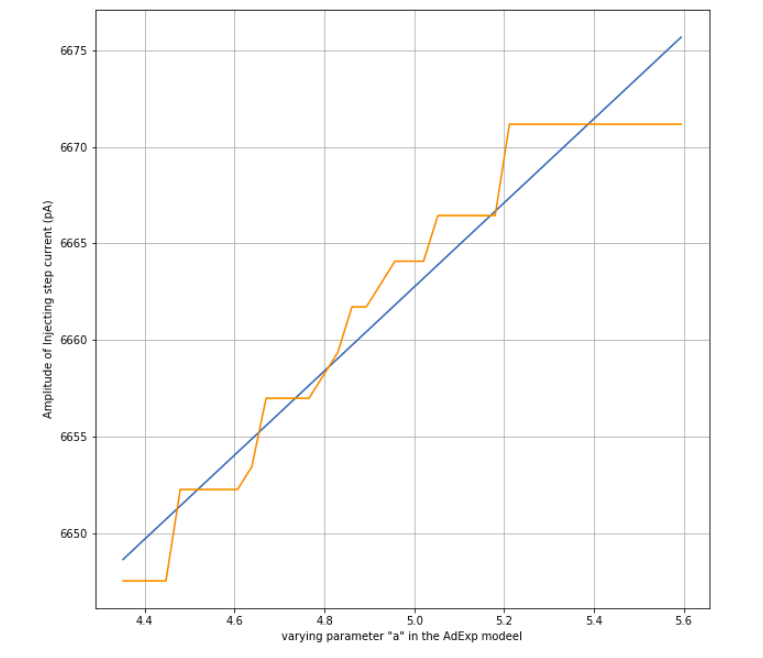
\includegraphics[]{figures/fundamental_cause_of_corrogations.png}
\caption[Causes of corrugation (1)]{\textbf{The Causes of Corrugation in Error Surfaces: Part A}.
I identified the main cause of corrugated error surfaces by re-calculating feature values as single parameters were varied.
Here, I vary parameter $a$ in the AdEx model.
The orange trace shows the computed rheobase current as this parameter is varied.
Note that it grows in a step-like manner, not according to the smooth linear fit (blue).
During periods when the rheobase is not increasing (but the parameter value is), the parameter may cause some other feature, computed at rheobase to vary in one direction.
Once the rheobase jumps, the stimulus used to compute the feature has changed, so that same feature may vary in the other direction.
Consequently, a computed feature-value may zig-zag, rather than exhibiting a smooth change, as a parameter is varied.}
\label{fig:corrugation-cause-1}
\end{center}
\end{figure}

Below I show a more concrete example of the same phenomena.
\begin{figure}
\begin{center}
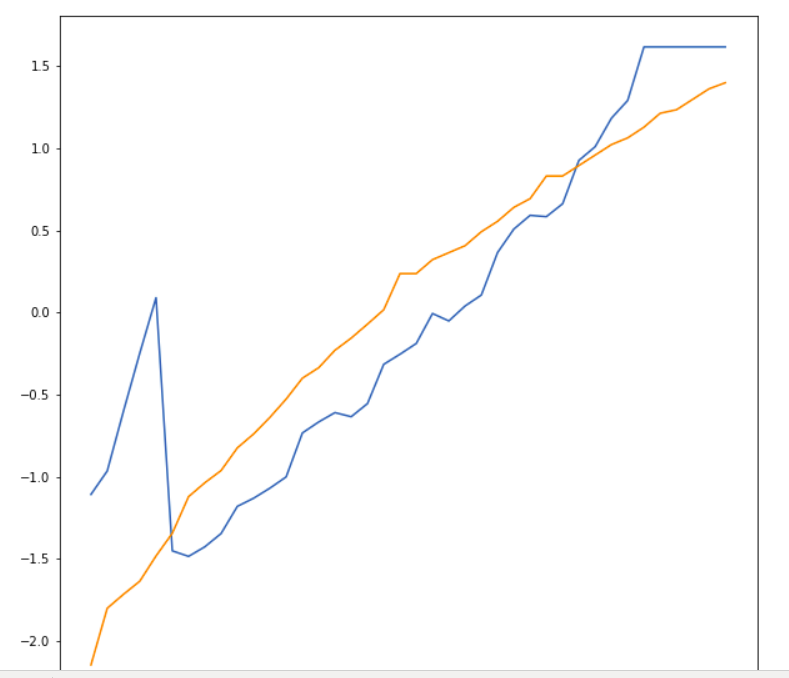
\includegraphics[]{figures/rh_vs_vt.png}
\caption[Causes of corrugation (2)]{\textbf{The Causes of Corrugation in Error Surfaces: Part B}.
Using an Izhikevich model, I vary a single odel parameter ($a$) as in Figure \ref{fig:corrugation-cause-1}, and plot the rheobase current (orange, normalized to its mean value) but also compute the value of the spike threshold (blue, also normalized).
Note the non-linear behavior of the response of this feature value to the change in the model parameter.
This non-linear behavior is mainly driven by a change in the amplitude of the injected current used to evoke it (the rheobase current), and not to underlying non-linearity in the location of the spike threshold for a fixed current.}
\label{fig:corrugation-cause-2}
\end{center}
\end{figure}

This can also be visualized in the waveforms themselves.
In Figure \ref{fig:variable-vt} the location (in time) of the threshold relative to the peak of the action potential varies in unpredictable ways as a single parameter of the model is increased.

\begin{figure}
\begin{center}
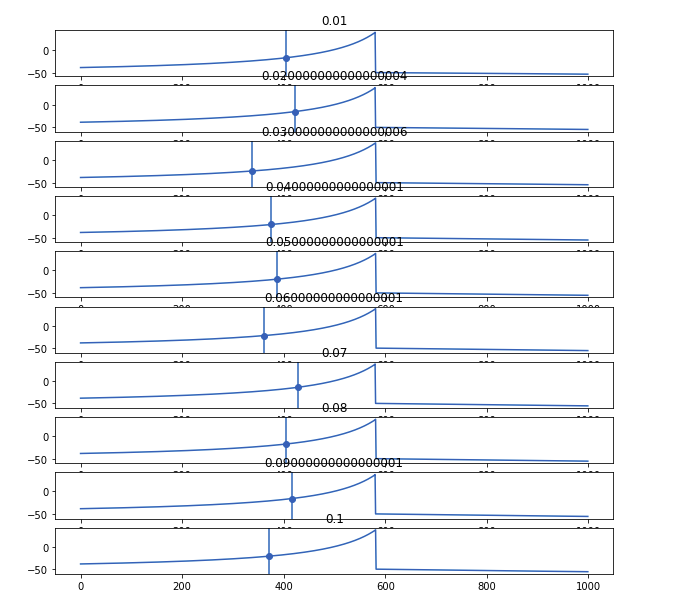
\includegraphics[]{figures/variable_vt.png}
\caption[Causes of corrugation (3)]{\textbf{The Causes of Corrugation in Error Surfaces: Part C}.
In order to see this effect directly in the responses themselves, I plot the action potential waveforms for the Izhikevich model as the value of parameter $a$ increases in small steps from the bottom panel to the top panel.
At each value of this parameter, rheobase is computed and the waveform of the spike evoked at rheobase is extracted.
Each such spike is aligned across panel, so that differences in the lead up to that spike can be examined.
The spike threshold, identified by the moment when the slope of the membrane potential reaches a target value, is shown with each blue dot, and the time that the threshold is reached is indicated by each vertical line.
It is clear that while the time of the threshold changes as $a$ is varied, it does not do so systematically.
Therefore the resulting error surface will not be useful for optimization.
This demonstrates that making features contingent upon the responses to the rheobase current results in major challenges to optimizaton.}
\label{fig:variable-vt}
\end{center}
\end{figure}

%An izhikevich model is used to examine the effects of sweeping across changes to parameter 'a' while retaining all other paramters as constant, on the plot, rheobase is and $V_{T}$ is calculated for each different value of 'a' and plotted on the same y-axis. It becomes apparent that rheobase (the orange trace) has minor zig-zags in its value, while $V_{T}$, has bigger and more significant zig-zags in its error, at this point all we have done is slowly varied and calculated $V_{T}$ but we have not plotted $V_{T}$ in relation to APs

% If all other conditions are favorable , as the remaining objective functions may have high fidelity; 

\subsubsection{Overcoming Contingent Discontinuities}
With sufficient care taken to avoid too many corrugations in the error surface,  optimization can still be viable.
However, this may mean discarding otherwise useful features that could in principle distinguish between competing regions of parameter space.
An alternative approach is to discard the rheobase entirely as a contingency,
making tests depend not on the rheobase value obtained from each parameterization of the model, but on the rheobase observed in the experimental data itself.
In other words, if the rheobase of the biological neuron is 100 pA, then the $1.5\times$ rheobase ISI test should be performed with a current injection of 150 pA, even if the rheobase of the current model parameterization is some entirely different value.

Another approach is to dispense with the rheobase entirely, and simply test using a fixed set of current amplitudes that span the suprathreshold portion of the F-I curve, e.g. 200pA, 350pA, and 500 pA for a typical neuron.
This seems extremely direct, but it in some cases it fails to explore the most interesting peri-threshold portion of the F-I curve, where the dynamics of single spikes contain a great deal of information about peri-threshold dynamics.
For example, an after-hyperpolarization that is visible after single spike at rheobase may become completely swamped by the combination of inward pipette current and sodium current at values of injected current that are high above threshold.

\subsection{Does a Genetic Algorithm adequately Report the Contours of the Error Surface?}
The error surface is vast, corresponding to all possible combinations of parameters at infinite resolution.
Naturally, this is only sparsely and strategically sampled.
Consequently there is no guarantee that it is has been adequately explored, and that lower error parameter sets do not exist somewhere that the optimizer did not adequately explore.

Next I describe how to visibly ``clean" corrugations from the error surface when using an approach based on a small list of non-contingent errors vs an alternative approach using models whose measurements are contingent on parameter dependent current values.

For each model a current is found that forces the model to fire at 12 spikes. Although not the exactly the same as rheobase, the algorithm is structurally identical, and the problems are the same. When eliciting a pre-determined spike count for any model parameterization (1 or x). This algorithm has the same propensity as the rheobase algorithm to introduce small current excesses into readings of subsequent tests, in this case EFEL tests of spike train shape.
%Because the rheobase algorithm is essentially an algorithm that searches %multiples of the experimentally observed rheobase.
Figures \ref{fig:constant_current} and \ref{fig:real_problem_nontrivial_surface-1} below show error surfaces from each paradigm.
Each of these figures depicts a heatmap of a 2D cross-section of the error surface.
The sensitivity of the objective function to systematic changes (grid search) of two parameters, centered around the optimizer's own solution, was explored.
All other parameters were held constant at the optimal values.
This effectively depicts a cross-section of the error surface near that solution.

%Case 1, Izhikevich model at threshold virtual experiment. Constraints used:
%\begin{table}
%\begin{tabular}{c}
%    TimeConstantTest \\
%    RestingPotentialTest \\
%    InputResistanceTest \\
%    CapacitanceTest \\
%    FITest \\
%\end{tabular}
%\caption[Izhikevich model rheobase constraints]{}
%\label{izhi-rheobase-constraints}
%\end{table}

%The surface plot from the supra threshold paradigm shows more contrast for two reasons: 1, it has less intermediary values (light green colour), reason two, it less high frequency changes, or ripples in the error surface.  

\begin{figure}
    \centering
    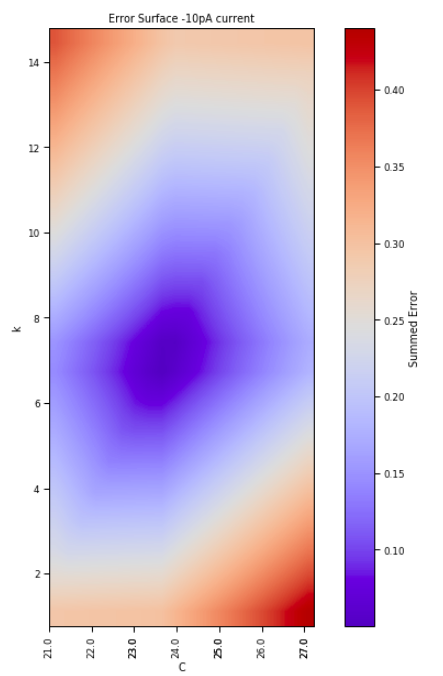
\includegraphics[scale=0.7]{figures/friendly_error_surface.png}
    \caption[Constant Currents Produce Tractable Error Surfaces]{\textbf{2D cross-section of the error surface for an Izhikevich model with no Contingent Tests}.
    The model was optimized against simulated data using 5 features.
    Any other features whose calculation is contingent on the rheobase were deliberately excluded.
    A 2D grid search was then applied (for parameters $C$ and $k$) around the resulting optimal set of parameters in order to visualize the local error surface.
    Although only 2 dimensions are explored here, there is no evidence of corrugation in this error surface, indicating that manageable, convex error surfaces can be realized when contingencies are removed.}
    \label{fig:constant_current}
\end{figure}

%\begin{figure}
    %\centering
 %   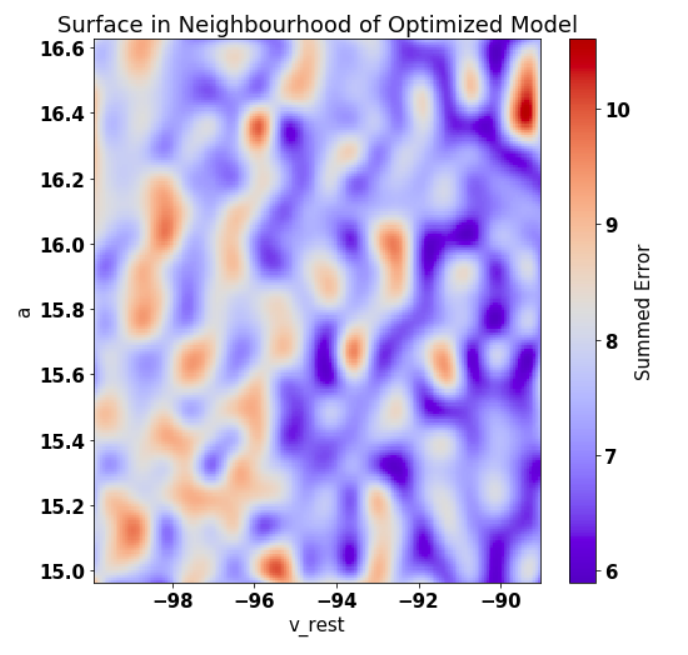
\includegraphics[scale=0.75]{figures/corrogated_surface_but_functional.png}
%\end{figure}  
\begin{figure}
    \centering
    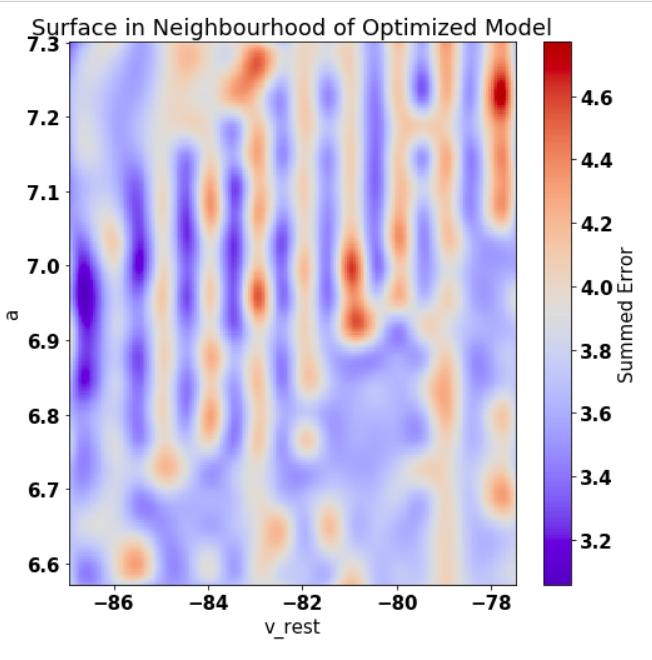
\includegraphics[scale=0.75]{figures/corrogations.png}
        \caption[A Complicated Error Surface]{\textbf{2D cross-section of the error surface for an AdEx model using EFEL features.}
    Similar to Figure \label{fig:constant_current}, except using an AdEx model and all 14 EFEL features.
    Despite lacking contingent tests, the error surface is still complex and Rastrigin-like.
    This shows that even removing contingent tests will not result in convex error surfaces for all combinations of models and tests.}
    \label{fig:real_problem_nontrivial_surface-1}
\end{figure}

%\begin{figure}
%    \centering
%    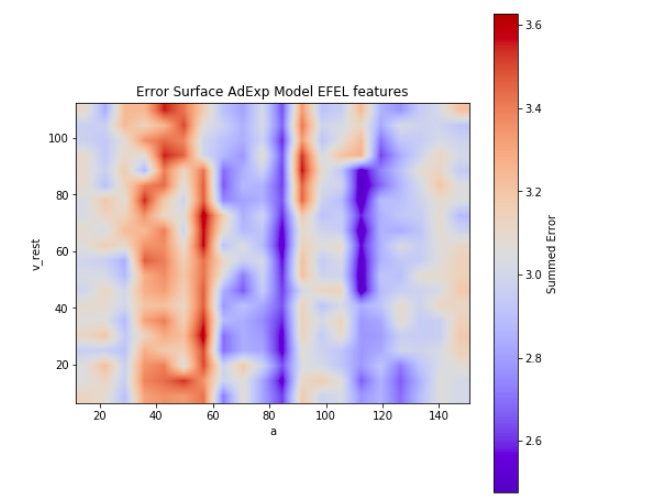
\includegraphics[scale=1.25]{figures/third_error_surface.png}
%    %\caption[Cliff ledge in 2D error surface]{Cliff ledge in 2D error surface}
%        \caption[Complex but not hopeless error surfaces]{Complex error surface %with alternating neighbouring ridges and valleys (ripples)}
%    \label{fig:real_problem_nontrivial_surface-2}
%\end{figure}

%%% . 
%The surprising complexity of these error surfaces did not become apparent to me until I had worked on this project for a few years. Its more complicated than that, I had evidence of complex surface since begining. We were dismissing as bug, as we did not conceptualize where these complex surfaces where coming from. Search slack, there are pictures of complex surfaces, since just after I started working on the project. I think the real problem is we were too confident in the first established NU tests, they where passing unit tests, which was good, but we should not have assumed they were conceptually sound to use in optimization.

%%%
I suspect that other pre-existing optimizers that aim to fit neuronal models are largely ignorant of the error surface they face.
In fact, without comprehensive data about the convergence rates of various competing approaches to optimization, we cannot now how efficiently each obtains its solutions, nor about alternative solutions that may have been missed.

Nonetheless, I am confident that genetic algorithms (in general) are preferable to to exhaustive search (which is impractical for all but the smallest models) and to gradient-descent-like approaches (due to the nature of the error surface).
However, successful optimization may require periodic exhaustive, local grids searches of the parameters space near the optimized values, in order to evaluate whether the error surface was tractable in the first place.
% NB, this is harder to understand than the residual rheobase error idea.    
% dont need to share complexity with reader.
%Although not shown here a third case is worth describing, as this third test combination achieved many useful results: Izhikevich model at threshold virtual experiment. Constraints used:
%\begin{verbatim}
%Case1 + RheobaseTest,
%\end{verbatim}

\section{Satisficing vs Optimizing}
%Genetic algorithms are favorable because they provide a good solution to the exploration/exploitation trade-off.
Unless hunting for a new prime number, few are willing to run compute jobs lasting for months, thus there are steeply limited budgets for exploring solution spaces. It therefore seems prudent to accept solutions which are are not optimal but are ``good enough", especially if these solutions can be obtained in a small fraction of the time.
Not all real neurons, even of the same nominal type, have identical properties, so perhaps we should embrace such variability in optimization results as well.
If the highest objective is to recover biologically plausible models, and many fitted models can easily meet this objective, then weaknesses in the ability of the optimizer to succeed in identifying the exact optimum in a very complex error surface can be tolerated.

Fortunately the coupling of Neuronunit to a Genetic Algorithm facilitates either optimizing or ``satisficing" as appropriate.
The term ``satisfice" means that a measured property is either deemed optimal or merely satisfactory \citep{simon1956rational}.
Although we may not know if a true optimum has been achieved, by using NeuronUnit in the evaluation, we can determine if the result is satisfactory enough, and then terminate optimization early.
This could be done by tracking the $\chi^2$ statistic during optimization and ending as soon as it drops below a certain level.
